\documentclass[american]{rtxreport}

\usepackage{listings}
\usepackage[utf8]{inputenc}

\author{David Pineau}
\title{Technical Documentation}

\rtxdoctype{Technical Documentation}
\rtxdocref{technical\_documentation}
\rtxdocversion{0.3}
\rtxdocstatus{Release}

\rtxdochistory{
0.1 & 10/03/2011 & David Pineau & Plan of the Technical Documentation \\
\hline
0.2 & 11/03/2011 & David Pineau & Chapters 1 to 3 done Intro and Chapter 4 still missing \\
\hline
0.3 & 11/03/2011 & Louis Opter & Cosmetic improvements \\
}

\newcommand{\note}[1]{\marginpar{\scriptsize{\textdagger\ #1}}}



\definecolor{lstbackground}{rgb}{0.95, 0.95, 0.95}
\definecolor{lstcomment}{rgb}{0, 0.12, 0.76}
\definecolor{lstkeyword}{rgb}{0.66, 0.13, 0.78}
\definecolor{lststring}{rgb}{0.67, 0.7, 0.13}
\definecolor{lstidentifier}{rgb}{0.1, 0.1, 0.1}

\lstset{
        tabsize=2,
        captionpos=b,
        emptylines=1,
        frame=single,
        breaklines=true,
        extendedchars=true,
        showstringspaces=false,
        showspaces=false,
        showtabs=false,
        basicstyle=\color{black}\small\ttfamily,
        numberstyle=\scriptsize\ttfamily,
        keywordstyle=\color{lstkeyword},
        commentstyle=\color{lstcomment},
        identifierstyle=\color{lstidentifier},
        stringstyle=\color{lststring},
        backgroundcolor=\color{lstbackground}
}

\definecolor{grey}{rgb}{0.90,0.90,0.90}
\definecolor{rBlue}{rgb}{0.0,0.24,0.96}
\definecolor{rRed}{rgb}{0.6,0.0,0.0}
\definecolor{rGreen}{rgb}{0.0,0.4,0.0}

\lstdefinelanguage{rtx}%
{
	morekeywords={DECLARE, SEQUENCE, INTERFACE, IMPLEMENTATION, FROM, READ,
        OPTIONAL, CONFIGURATION_VARIABLE, USE, AS, WITH, SEQUENCES, ON, ELSE,
        LET, PROVIDES, REQUIRE, THROWS, FINALLY, FOREACH, IN, AND, OR, THROW,
        HANDLE_ERROR, NOT, REGISTER, LIKE, BIT, INTEGER, DOUBLE, BOOLEAN,
        STRING, MAPPED_AT, PCI},%
	sensitive=true,%
	morecomment=[l][\color{rRed}]{//},%
 	morecomment=[l][\color{rRed}]{\#},%
	morecomment=[s][\color{rRed}]{/*}{*/},%
	morestring=[b][\color{rGreen}]",%
	morestring=[b][\color{rGreen}]',%
	keywordstyle={\color{rBlue}}%
}[keywords,comments,strings]

\lstdefinelanguage{rti}%
{
	morekeywords={interface,
        builtin,
        type, sequence, variable,
        provided, required, optional},%
	sensitive=true,%
	morecomment=[l][\color{rRed}]{//},%
 	morecomment=[l][\color{rRed}]{\#},%
	morecomment=[s][\color{rRed}]{/*}{*/},%
	morestring=[b][\color{rGreen}]",%
	morestring=[b][\color{rGreen}]',%
	keywordstyle={\color{rBlue}}%
}[keywords,comments,strings]

\lstdefinelanguage{blt}%
{
	morekeywords={template,
        decl, stmt},%
	sensitive=true,%
	morecomment=[l][\color{rRed}]{//},%
 	morecomment=[l][\color{rRed}]{\#},%
	morecomment=[s][\color{rRed}]{/*}{*/},%
	morestring=[b][\color{rGreen}]",%
	morestring=[b][\color{rGreen}]',%
	keywordstyle={\color{rBlue}}%
}[keywords,comments,strings]





\begin{document}

\maketitle

\rtxmaketitleblock

\tableofcontents

\begin{abstract}
    This document describes how the \rtx\ compiler works, starting with the
    different steps of the compilation process, up to how it is implemented.
\end{abstract}


%\section*{Introduction}
%% What is Rathaxes
%% What is this document about exactly



\chapter{The tools that constitute \rtx}

\section{The language: CodeWorker}

\emph{CodeWorker} is an Open Source parsing tool and a source code generator
devoted to generative programming made by Cédric Lemaire. Generative
programming is a software engineering approach interested in automating the
production of reusable, tailor-made, adaptable and reliable IT systems. In
layman's terms, \emph{CodeWorker} lets you generate code by parsing existing
languages, or by creating and parsing your own language. We will be using it
for this exact purpose as ``a compiler of compilers''. Once a language file has
been parsed, CodeWorker provides several techniques for generating code.

The tool's scripting language drives the parsing and source code generation
process. Its syntax is derived from the C family of languages, making it
familiar to most programmers. The template syntax is like JSP, ASP, or
Velocity. It has variations for parsing, code generation, or procedural
programming, giving the developer a number of options for organizing
\emph{CodeWorker} projects. 

\emph{Codeworker} is more powerful and easier to use than \emph{Lex/Yacc},
\emph{CodeWorker} perfectly fits \rtx' code generation needs. It can be
divided into three major parts:

\begin{itemize}
    \item \emph{BNF} description language: \emph{Codeworker}'s parsing language
        requires a simple \emph{BNF} description of the language to parse, and
        each \emph{BNF} Rule is overloadable for extension purposes. The DSL of
        \rtx\ will be described thus.
    \item Scripting language: Codeworker scripts are
        powerful enough for the tree decoration needs of \rtx.
    \item Generation scripting language: We will then use the templating
        functionalities of CodeWorker to generate C code.
\end{itemize}



\section{The CNorm library}

\emph{CNorm} is a C parsing tool written with \emph{CodeWorker} made by Lionel
Auroux (Epita/Epitech system \& security laboratory's director), Cédric Lemaire
(CodeWorker's author and developer) and David Giron, David Amsallem and
Christophe Fajardo (all from the 2009 \rtx\ team). It also contains

This parser has been designed to be as powerful as possible to be able to
parse any dialect of C (extensions with specific qualifiers and specifiers).

\begin{itemize}
    \item Standard C 89 syntax
    \item GnuC asm expressions
    \item GnuC \texttt{\_\_thread} storage class specifier
    \item GnuC parameter forward declaration
    \item GnuC \texttt{\_\_extension\_\_} avoids warnings on GnuC extensions
    \item GnuC subscript
    \item GnuC designated initializer
    \item GnuC \texttt{\_\_builtin\_offsetof}
    \item GnuC \texttt{\_\_builtin\_va\_list}
    \item c99 \texttt{static} in direct absolute declarator
    \item c99 block as single expression (\texttt{\{ \}})
    \item c99 \texttt{typeof}
    \item c99 designation
    \item c99 \texttt{\_\_alignof}
    \item c99 \texttt{complex}, \texttt{\_\_real} \& \texttt{\_\_imag operator}
    \item c99 range expression
    \item c99 and Windows attributes
    \item K. \& R. coding style
    \item Missing type in function declaration
\end{itemize}

This grammar was adapted from the one in section A13 of the C programming
language, second edition, by Brian W. Kernighan and Dennis M. Ritchie
(Englewood Cliffs, New Jersey: Prentice Hall PTR, 1988; ISBN 0-13-110362-8),
pages 234 - 238. 

Cnorm is used in \rtx\ to parse the C code present in the BDSL in order to
avoid opaque datas and to provide full control on the handled code. It is also
used for the final C driver code generation. The C abstract syntax tree
organisation ca be found in Cnorm's own documentation. It won't be covered by
this one.



\chapter{Use cases of the compiler}

\section{Who will use \rtx}

As described in the Introduction, \rtx\ is aimed at two kinds of developers.

The primary target is the device driver developer. He will write a code
describing the algorithms to implement for the specific device he's writing
the driver for.

The secondary target is the kernel developer. His role is to implement the
template library that contains a templated C code containing the
OS-specific code.

Finally, a third kind of developer will have yet another role in the
development of a device driver. Using a ``State Of the Art'' of writing a
driver, he will design an interface that both the kernel developer and
the device driver developer will have to follow in their codes.

\section{The three parts of the DSL}

As you can see, three kinds of users and developers will interact with \rtx,
and make it evolve, each focused on a specific part of the DSL.
Each one of those three parts has its own place and function in the process of
compiling a \rtx\ driver.

\subsection{\rtx\ Maintainer: the Middle-End}
\lstset{language=rti}

First and foremost, although not really the first visible kind of contributor
to the language, is the \rtx\ maintainer. As described earlier, his role is
to design an interface that will have to be respected by both of the other kinds
of developer that will use our compiler and code in \rtx.

Those interfaces are part of what we will now call the \emph{Middle-End} of the
language. It could be seen as an compiler-internal description of what is
required or optional for both the driver's code and the template code
implementation. That will be the link between the \emph{Front-End} and the
\emph{Back-End}, by defining the available types, sequences and variables.

The file extension for this part of the DSL is \texttt{.rti} (\rtx\ Interface).

It is identified by an unique name in the compiler, generally identifying the
kind of sub-system it is created to describe.

It contains:
\begin{itemize}
    \item The types that are used in the sub-system, that must be provided by
        the template C code;
    \item The sequences (functions or algorithms) that are provided by the
        template C code;
    \item The sequences (functions or algorithms) that are required
        (they can be optional) from the device's \rtx\ driver;
    \item The configuration variables/values needed by the interface.
\end{itemize}

For example, we could have:
\begin{itemize}
    \item Userland interface: describes the \emph{LKM}'s functions and types;
    \item PCI interface: describes the PCI BUS function's and types;
    \item IO interface : describing the functions that can be used
for a device driver which device is on the IO port.
\end{itemize}

Here is an example of what an interface can look like:
\begin{lstlisting}
    interface Userland
    {
        // Here a list of compiler-builtin types
        builtin type bit;
        builtin type byte;
        builtin type word;
        builtin type dword;
        builtin type qword;

        builtin type register;
        builtin type buffer;
        builtin type context;

        // Here a type that has to be implemented in the templates
        type device;

        // Here is a sequence provided by the templates
        provided sequence concat(register, buffer);

        // Here are the sequences asked from the .rtx file
        required sequence doSomething(context, register);
        optional sequence doNothing(device);

        // Here the variables required from the .rtx file
        required variable os;
        required variable version_major;
        optional variable version_minor;
    };
\end{lstlisting}

Actually, this part of the DSL is the only one that doesn't need anything else
apart its dependencies to be checked as a valid code. In fact it is this part
that defines any generic type to be used in any other \rtx\ code.

\subsection{Kernel Developer: the Back-End}
\lstset{language=blt}

Secondly, another unavoidable kind of contributor to \rtx\ is the Kernel
Developer. This is them who will implement the backend library in order to add
the support of a new Operating System in \rtx.

The role of the \emph{Back-End} is to provide the platform-specific code for
each part of the \rtx\ (and then final) driver. The file extension is
\texttt{.blt} (\emph{Back-End} Library Template).

By using the interfaces present in itself, the compiler will be able to tell
what is supported or not for a specific Operating System, as well as telling
whether the types are used wrongly or not in the template code.

The template code is contained in a \emph{with} block that associates the code
with specific configuration variables and values. This means that the template
will be used when those specific variables equal the associated values.

Inside the \emph{with} block can be found one or more templates of code. A
template of code is identified by its type. This is the part that allows
referencing or using templates from inside others.

The content of the template is actually some instrumentalized C code that may
(or may not) be platform-dependant. By instrumented is meant that a
\rtx-specific syntax extends the C in order to use \rtx\ template
variables inside the C. This syntax also allows the concatenation of strings
in order to craft identifiers.

Here is a little example of what it can look like:
\begin{lstlisting}
    with os=Linux, version >= 2.6, bus=ioport
    {
        template get(register reg) decl
        {
            ${register} get_reg_${reg.name}(void)
            {
                return in${reg.basetype.initial}(${reg.addr});
            }
        }

        template get(register reg) stmt
        {
            get_reg_${reg.name}()
        }
    }
\end{lstlisting}

\subsection{Device driver Developer: the Front-End}
\lstset{language=rtx}

Finally, the last and most obvious part of the DSL, the so-called
\emph{Front-End}. This is the part an electronics engineer or a driver
developer will use. This part of the language possesses a syntax that allows
describing the registers of a device, how to access them, how to manipulate
them, as well as describing the algorithms that will use the device. The file
extension used for this part of the language is \texttt{.rtx} (\rtx).

One of the most important aspects of the \emph{Front-End} is that it contains a
\emph{configuration} block. This block contains the declaration of what was
earlier called the configuration variables. Those variable alter the compilation
process of a driver.

Compiling a \texttt{.rtx} file means checking the types and the availability of
each type or sequence by checking each of them against the matching interfaces
from the \emph{Middle-End}. See section
\ref{sec:driverCompilation}



\chapter{Compiler Architecture} %% take the tex code out of the AA2 doc.

\section{The different modules of the compiler}

A compiler is never a simple program. In the case of \rtx, we can identify
different elements inside the core of the compiler. Since the flexibility and
scalability of the language is one of the side-goals of the project,
those modules were an absolute necessity. Here is the diagram showing them:

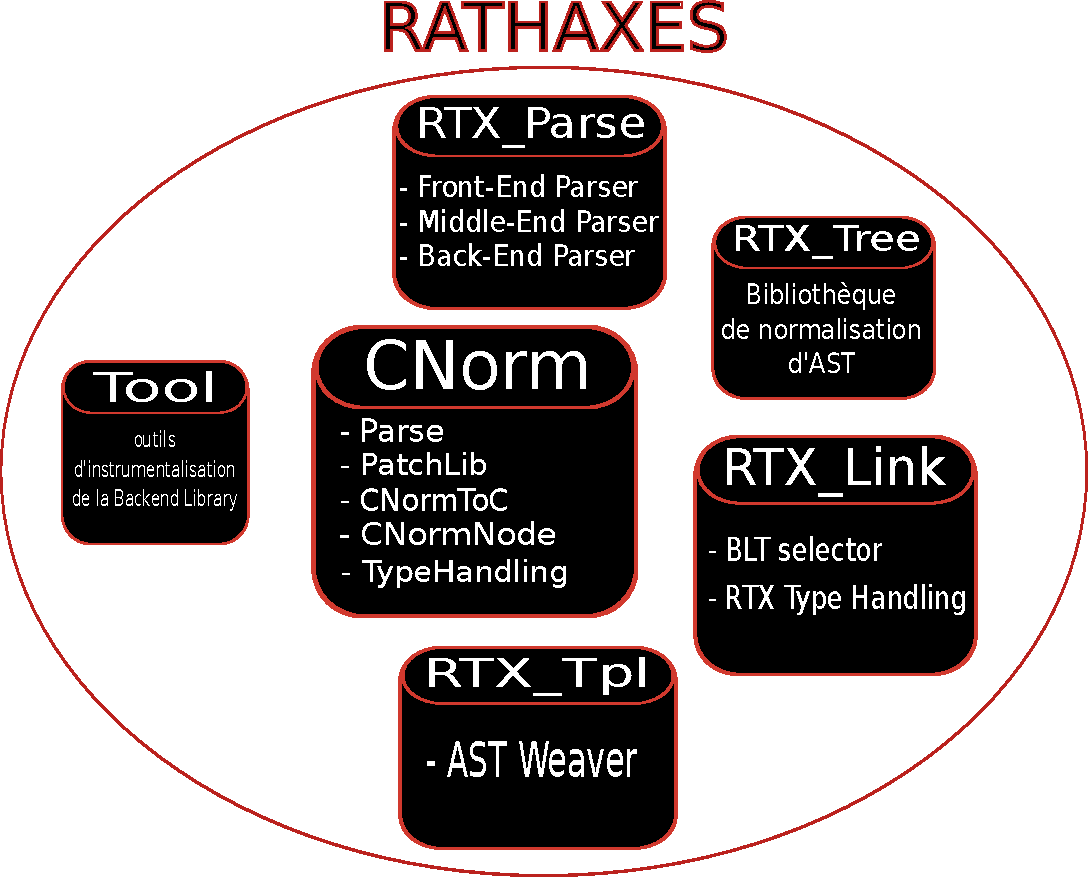
\includegraphics[width=0.95\textwidth]{diagramme_architecture.pdf}

First of all, the \emph{CNorm} library seen previously can be found inside the
compiler. Its role is firstly to generate the final C code, but it also allows
to parse C code. In the case of \rtx, it is overloaded in order to extend
the language and thus to easily parse the templated C code inside the DSL.

The next module, \emph{RTX\_Parse} is the part of the compiler which role is,
as its name implies, to parse the \rtx\ code and built a basic Abstract
Syntax Tree (AST) from it.

\emph{RTX\_Tree} comes with \emph{RTX\_Parse}, as it is a library that helps
normalizing the AST. This way, every type of node in it always respects a given
data representation.

Then, the two modules \emph{RTX\_Link} and \emph{RTX\_Tpl} are the modules that
enter in the process of transforming the raw AST by using the templates in
order to build a complete AST that can be outputted as C code. Their roles will
be detailed in the section \ref{sec:compilationSteps}.

Finally, the \emph{Tool} module, as its name implies, is a series of tools that
offer many kinds of possibilities. For example, a driver on an Unix system
needs a Makefile to be built, a driver on a Windows system need a \texttt{.inf}
file in order to be loaded, \ldots This module offers to generate these kinds
of files.


\section{The different steps of the compilation}
\label{sec:compilationSteps}

From the parsing of a \texttt{.rtx} file to the generation of the driver's C
code, the AST will undergo a number of transformations. However, the templates
of code are also compiled in order to allow caching in the core of the compiler.
That leads to two compilation schemes: a template's compilation and a driver's
compilation.

\subsection{Steps of a template's compilation}

The compilation of a template can be divided in many steps, since the template
code compilation generates an AST representation and a CodeWorker code that
will help integrate this AST generated from the template into the driver's AST.

We can then identify the following steps:
\begin{enumerate}
    \item Parsing: construction of an AST normalized by CNormNode and
        RTX\_Tree;
    \item Place Holders Identification: construction of a node containing
        every template placeholder;
    \item Place Holders Parsing: construction of an AST Node for each
        place holder;
    \item Code Generation: generation of CodeWorker code that resolves the
        linkage of the main AST with the template AST Node.
\end{enumerate}

Afterwards, the developer will be able to install the template into the Back-End
Library. Installing it means that an entry will be added into a specific
cache/registry of the compiler, that helps it associate the right templates to
a given driver at compile-time.


\subsection{Steps of a driver's compilation}
\label{sec:driverCompilation}

The compilation of a driver is a complex process, where every single part of the
DSL is taken in account.

Here is a short list of the steps of its compilation:
\begin{enumerate}
    \item Parsing: construction of an AST from the Front-End syntax;
    \item Type Checking: check of the types used in the Front-End against the
        types described in the Middle-End for validation;
    \item Template selection: the RTX\_Link module selects in the cache which
        templates to load for possible use by checking with the configuration
        variables;
    \item Template instantiation: the RTX\_Tpl module instantiates each
        template AST Node referenced by a Front-End AST Node, and calls the
        linkage resolver functions generated for the template AST Node.
    \item C Code Generation: Generation of the C code from the transformed
        AST;
    \item Utils Generation: the Tool module generates utility files like
        Makefiles for Unix or info files (\texttt{.inf}) for Windows modules,
        \ldots
\end{enumerate}


\subsection{General compilation process}

As you may have already understood, if we talked about three different parts
of the DSL, that means that it is one and only one language. Actually, one could
write a driver with the three parts in one same file. Although this is not
planned to be offered to driver or kernel developers, since their roles are
confined to one part of the language each, it is a possibility. The keywords
in the file will then tell which kind of compilation to activate.

Here is a schema picturing this general process:

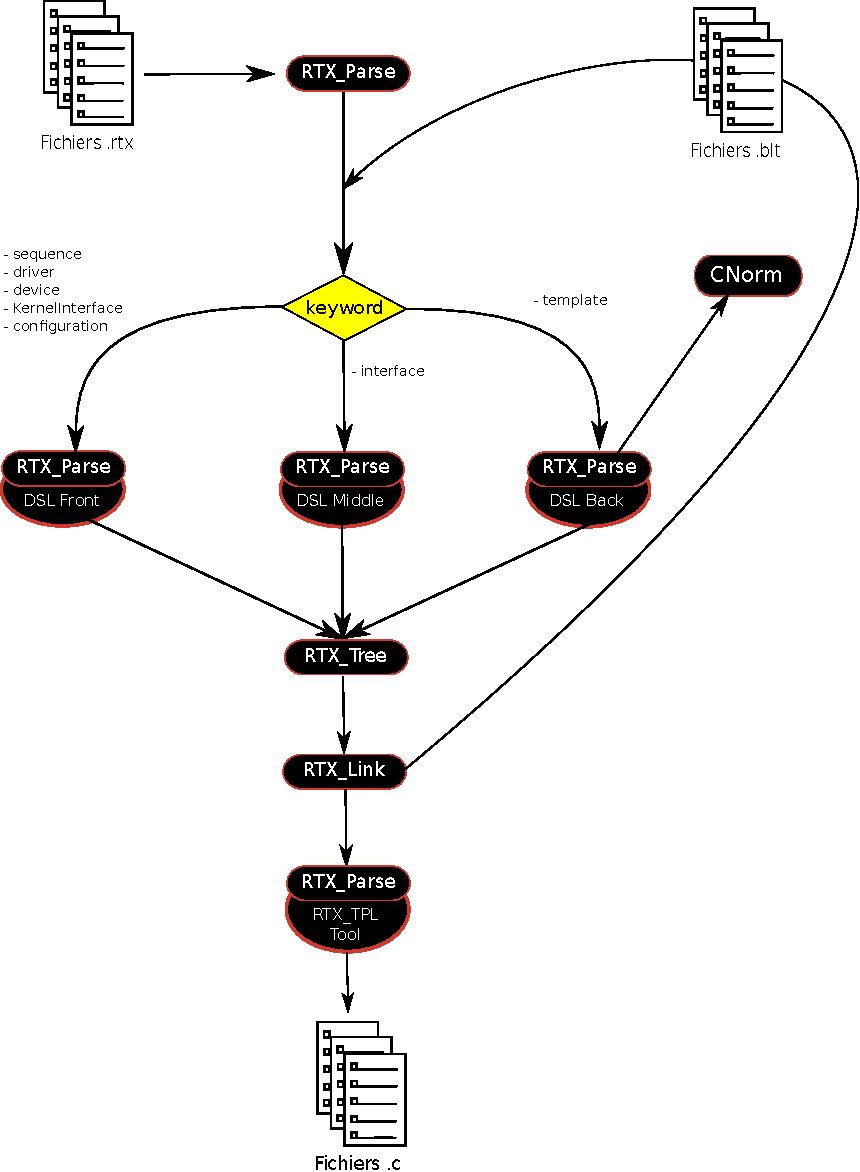
\includegraphics[width=0.95\textwidth]{logigramme.pdf}



\chapter{Details of implementation}




\end{document}
